\documentclass[tikz, border=2pt]{standalone}

\usepackage{amsmath,amssymb}
\usepackage{xcolor}

\definecolor{utnblue}{RGB}{0, 51, 102}

\begin{document}
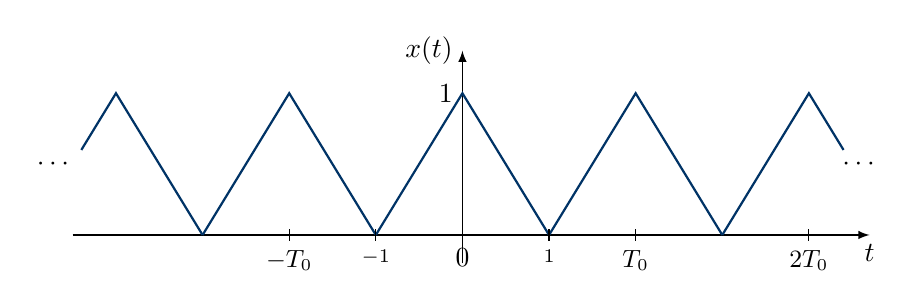
\begin{tikzpicture}[>=latex, xscale=1.1, yscale=1.8]
    % Eje
    \draw[->] (-4.5, 0) -- (4.7, 0) node[below] {$t$};
    \draw[->] (0, -0.2) -- (0, 1.3) node[left] {$x(t)$};

    % Triángulos: base 2, altura 1, centrados en 2k con T_0=2
    % Triángulo en t=-4
    \draw[utnblue, thick] (-5, 0) -- (-5, 0); % padding
    % Triángulo centrado en t=-2
    \draw[utnblue, thick] (-3, 0) -- (-2, 1) -- (-1, 0);
    % Triángulo centrado en t=0
    \draw[utnblue, thick] (-1, 0) -- (0, 1) -- (1, 0);
    % Triángulo centrado en t=2
    \draw[utnblue, thick] (1, 0) -- (2, 1) -- (3, 0);
    % Triángulo centrado en t=4
    \draw[utnblue, thick] (3, 0) -- (4, 1) -- (4.4, 0.6);
    % a la izquierda: continuación del triángulo en -4
    \draw[utnblue, thick] (-4.4, 0.6) -- (-4, 1) -- (-3, 0);

    % Marcas y etiquetas
    \node[below] at (0, -0.03) {$0$};
    \draw (-2, 0.04) -- (-2, -0.04) node[below] {\small$-T_0$};
    \draw (2, 0.04) -- (2, -0.04) node[below] {\small$T_0$};
    \draw (4, 0.04) -- (4, -0.04) node[below] {\small$2T_0$};
    \draw (-1, 0.04) -- (-1, -0.04) node[below, font=\scriptsize] {$-1$};
    \draw (1, 0.04) -- (1, -0.04) node[below, font=\scriptsize] {$1$};
    \node[left] at (0, 1) {$1$};

    % Puntos suspensivos
    \node at (-4.7, 0.5) {$\cdots$};
    \node at (4.6, 0.5) {$\cdots$};
\end{tikzpicture}
\end{document}
